% !TeX spellcheck = en_US
\section{Traditional Feature-Based Classifier}


\subsection{Feature Extraction}

Feature extraction is an essential component in audio analysis tasks, as it allows the transformation of raw audio data into a set of informative features that can capture key characteristics of the signal.

In this regard, the widely-used Librosa toolkit was employed to extract various audio features, which were subsequently processed using statistical metrics. The extracted features and associated metrics are summarized in Table \ref{table:extractedFeat}, having in total, extracted 327 features.

\begin{table}[h]
	\centering
	\caption{Extracted Audio Features and Statistical Functions Applied to Them}
	\label{table:extractedFeat}
	
	\begin{tabular}{@{}cc@{}}
		\toprule
		Audio Features & Statistical Functions \\
		\midrule
		&  \multirow{10}{*}{\begin{tabular}{@{}c@{}}Minimum\\Mean\\Maximum\\Median\\25th percentile\\75th percentile\\Spikes\footnotemark[1]\\Variance \\Standard Deviation\\Sum\\Kurtosis\footnotemark[2]\\Skew\footnotemark[2]\end{tabular}} \\
		\acp{mfccs} 1 - 21 & \\
		Mel Spectrogram & \\
		Root-Mean-Square & \\
		Chromagram & \\
		Spectral Centroid & \\
		Spectral Contrast & \\
		Spectral Bandwith & \\
		Roll-Off Frequency & \\
		Tonnetz & \\
		Zero-Crossing Rate & \\
		& \\
		\bottomrule
		\multicolumn{2}{l}{\footnotemark[1]\footnotesize{Custom function detailed on the Feature Selection section.}} \\
		\multicolumn{2}{l}{\footnotemark[2]\footnotesize{Only for the \acp{mfccs}.}} \\
	\end{tabular}
\end{table}

\subsection{Feature Analysis}

One important task following feature extraction is to analyze and interpret the extracted data to gain a deeper understanding of the audio signals and the features that describe them.

\subsubsection{Audio Signal Study}

In this process, we visually analyzed and interpreted the features' data by graphically representing each feature from an audio segment. The figures in Section \ref{sec:App:1} of the appendix demonstrate some of the graphics we used to visualize the data.

\subsubsection{Spikes Metric}

Initially, wave plots were observed, and we noted consistency in the number of high values. For this reason, we created a custom metric that calculates those high values, which we called "spikes", from the features' data.

In Figure \ref{fig:zcrSpikes}, it is possible to visualize the zero crossing rates' wave plots in different emotions. The horizontal line represents the threshold that we considered, any value above was considered to be a spike, which is annotated with red dots in the graphic. The threshold used was manually tested and obtained decent consistency of the number of spikes, within an emotion, by using the mean value of the feature plus 2\% of the standard deviation. Consequently, this metric was also tested and applied to every other audio feature.

\begin{figure}[H]
	\centering
	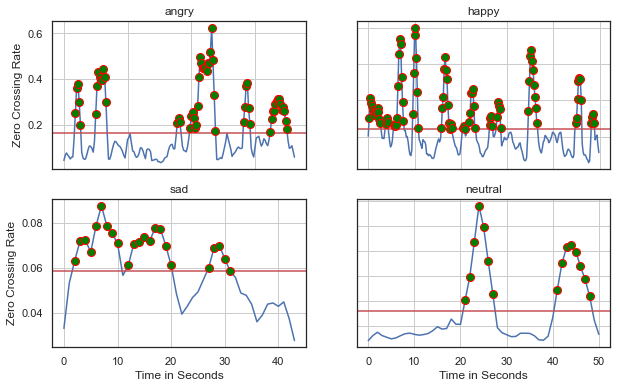
\includegraphics[width=\textwidth]{figs/4_1_traditional/zcr_waveplot_spikes.png}
	\caption{Zero crossing rate wave plot annotated with spikes.}
	\label{fig:zcrSpikes}
\end{figure}


\subsubsection{Bar Plots}

Furthermore, bar plots were useful for viewing the overall extracted features' data plainly and quickly, and to understand the numeric values of each feature and metric used on it.

For example, figure \ref{fig:melBarPlot} shows clear differences in the mean values for some metrics used on the Mel Spectrogram.

\begin{figure}[H]
	\centering
	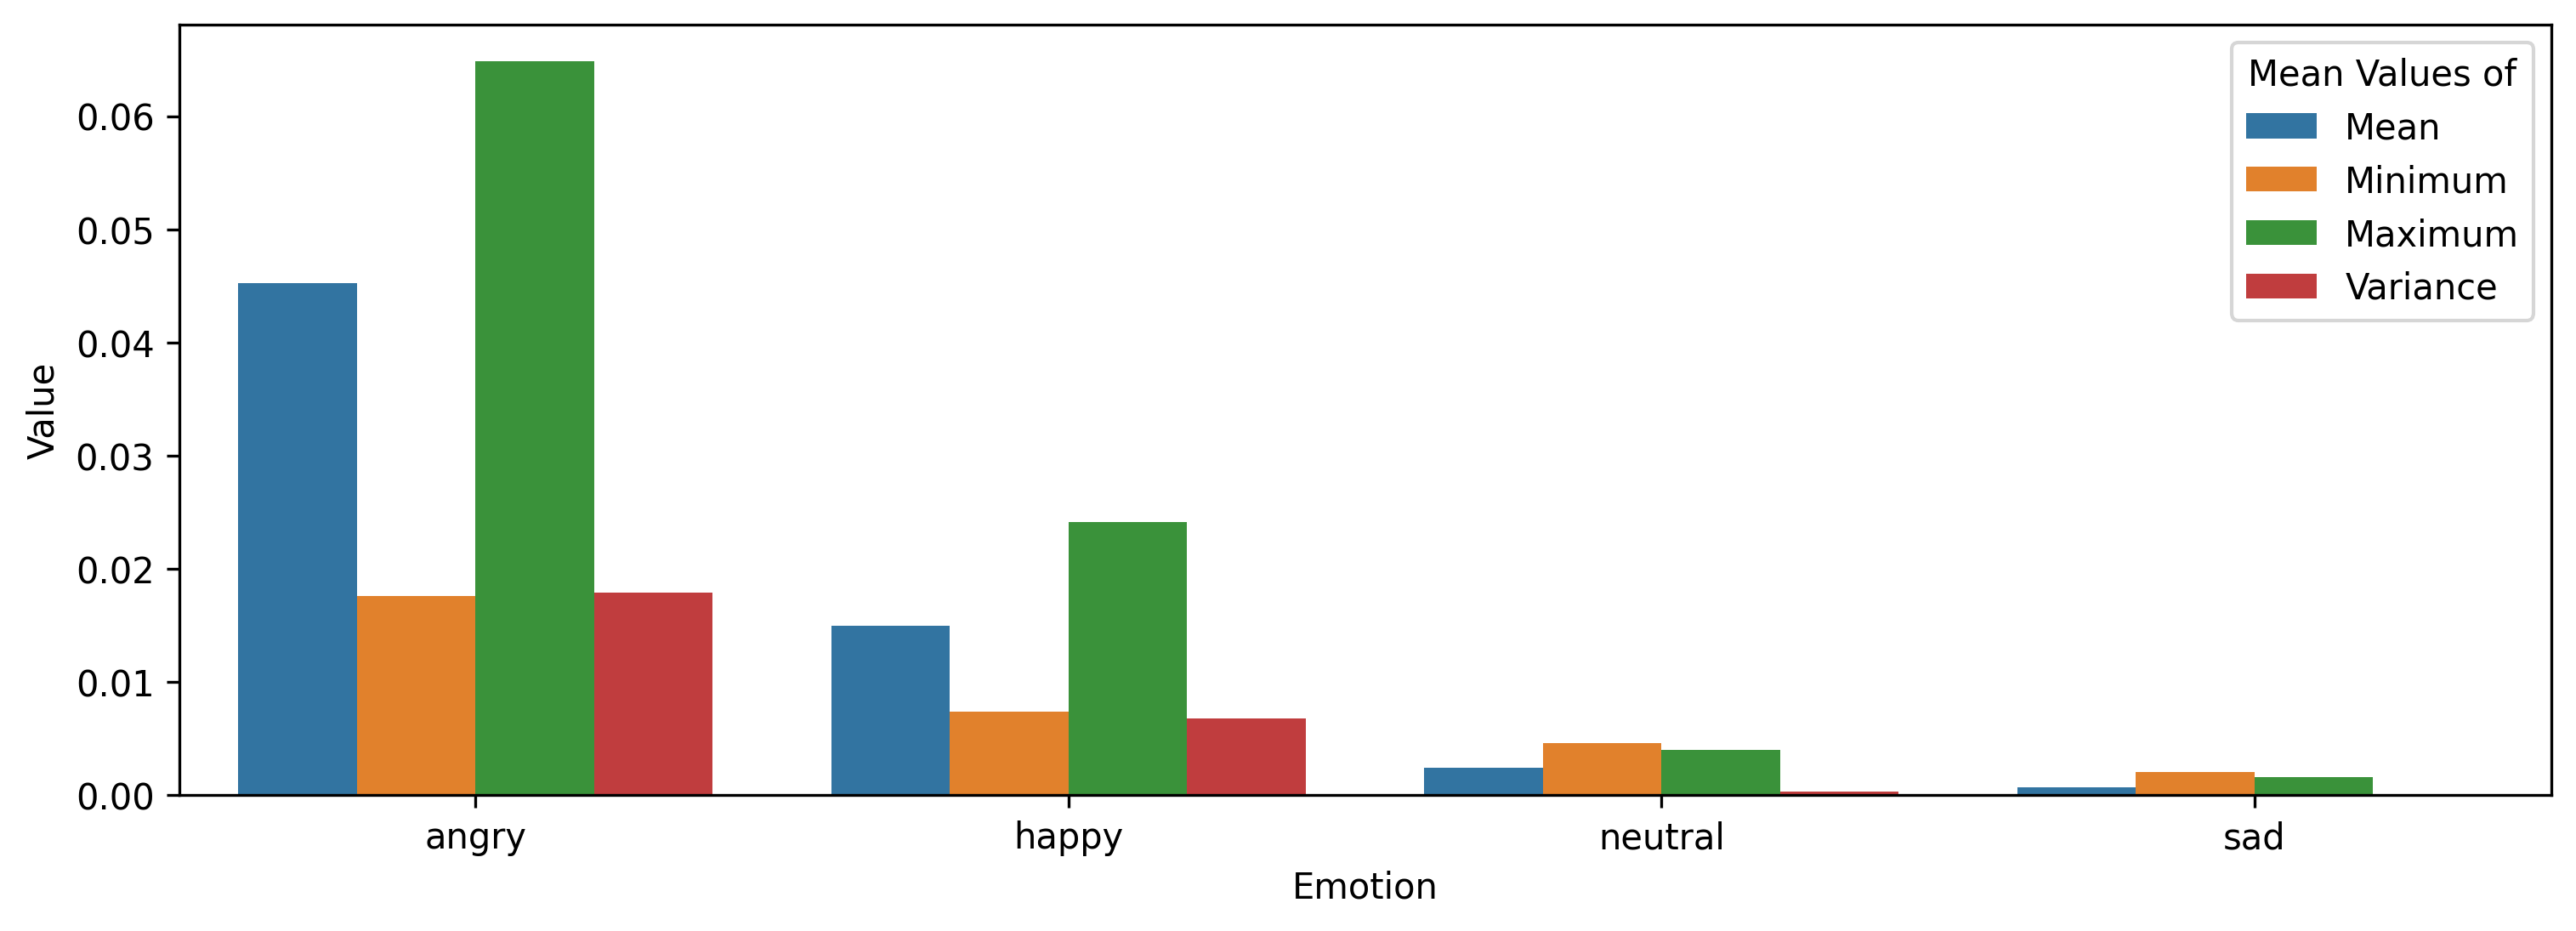
\includegraphics[width=\textwidth]{figs/4_1_traditional/meanFeatBarPlot.png}
	\caption{Bar plots mean for metrics used on the mel-scaled spectrogram feature}
	\label{fig:melBarPlot}
\end{figure}


\subsubsection{Wave Plots with Surrounding Areas}

During the feature study process, it was observed the wave plots of some features surrounded by a small area above and below the original wave (defined through a selected threshold). This was done to corroborate how well the feature describes different emotions. A high degree of overlap between surrounding areas of a feature on a given emotion for different subjects could indicate that the feature is relevant for representing that emotion.

The figure \ref{fig:zcrAreaOnly1} is an excerpt of the figure \ref{fig:zcrArea} in the appendix, and it demonstrates an example of this analysis for the zero crossing rate with 5 different subjects on the same sentence for the anger emotions.

From this graphic, it was observed that there is a sufficient amount of overlap between the surrounding areas for each emotion to conclude that the feature has some utility for describing each emotion. However, due to the different lengths of each audio segment, it is ambitious to guarantee this conclusion.

\begin{figure}[H]
	\centering
	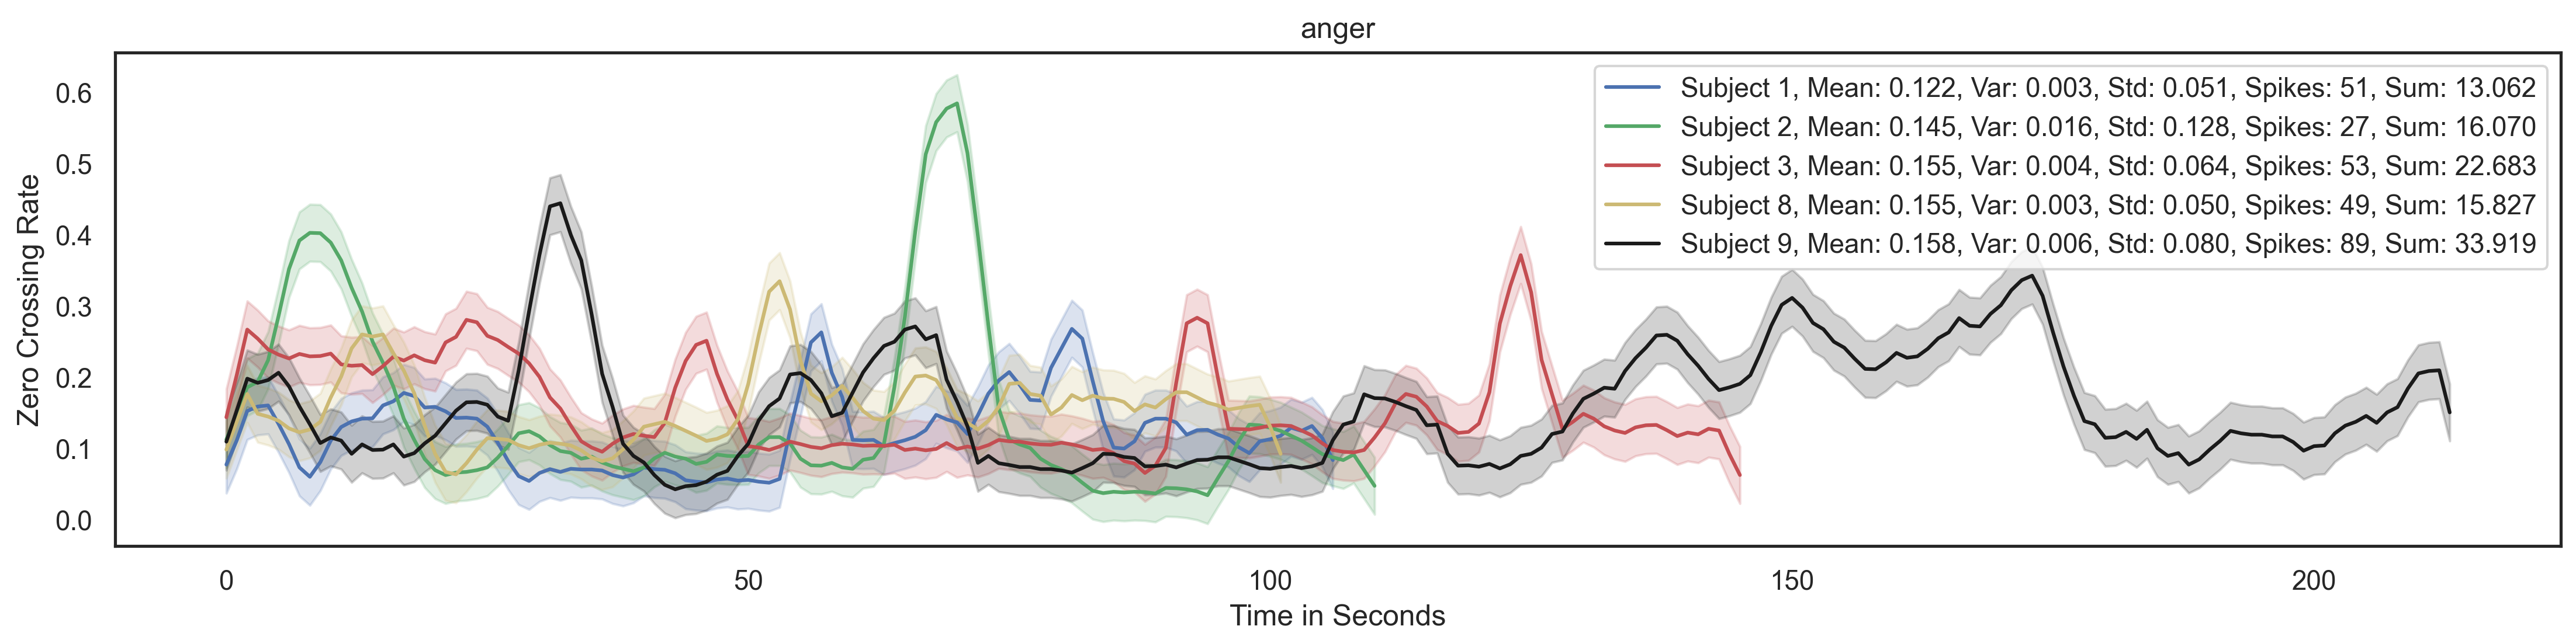
\includegraphics[width=1\linewidth]{figs/4_1_traditional/zcrAreaOnly1.png}
	\caption{Zero crossing rate wave plot with a surrounding area of five male subjects for the same utterance with the anger emotion.}
	\label{fig:zcrAreaOnly1}
\end{figure}

This same idea can also be used to determine whether a feature is favorable for creating a distinction between different emotions, which is naturally useful for the problem of classifying emotions. The conclusion can be drawn by observing the opposite of the previous example. If the areas around the zero crossing rate do not coincide too heavily, it is an indicator that the feature could be adequate for distinguishing different emotions.

Figure \ref{fig:zcrAreaSameSubj} displays six zero crossing rates of one subject saying the same sentence but expressing different emotions. As previously mentioned, since audio lengths are different, it is difficult to draw a direct and well-founded conclusion.

\begin{figure}[H]
	\centering
	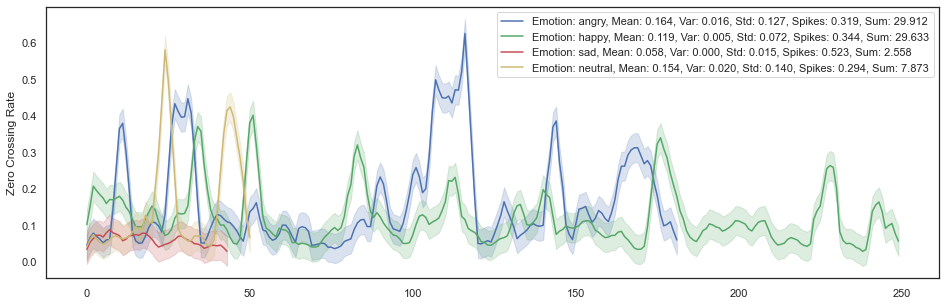
\includegraphics[width=\linewidth]{figs/4_1_traditional/zcr_male_same_subject.png}
	\caption{Zero crossing rate wave plots with a surrounding area of a single male subject and sentence for all different emotions.}
	\label{fig:zcrAreaSameSubj}
\end{figure}

Overall, this approach of surrounding wave plots with areas provided us valuable insight into the ability of a feature to describe and distinguish emotions, though it is a little limited by the varying lengths of audio segments.

\subsubsection{Variation Plots}

Another graph made was a variation plot, to perceive the differences in the features' values, across several audios for the same emotion. Figure \ref{fig:zcrMeanVar} shows an example of this type of plot for the mean zero crossing rate value across 50 speech utterances for all emotions.

\begin{figure}[H]
	\centering
	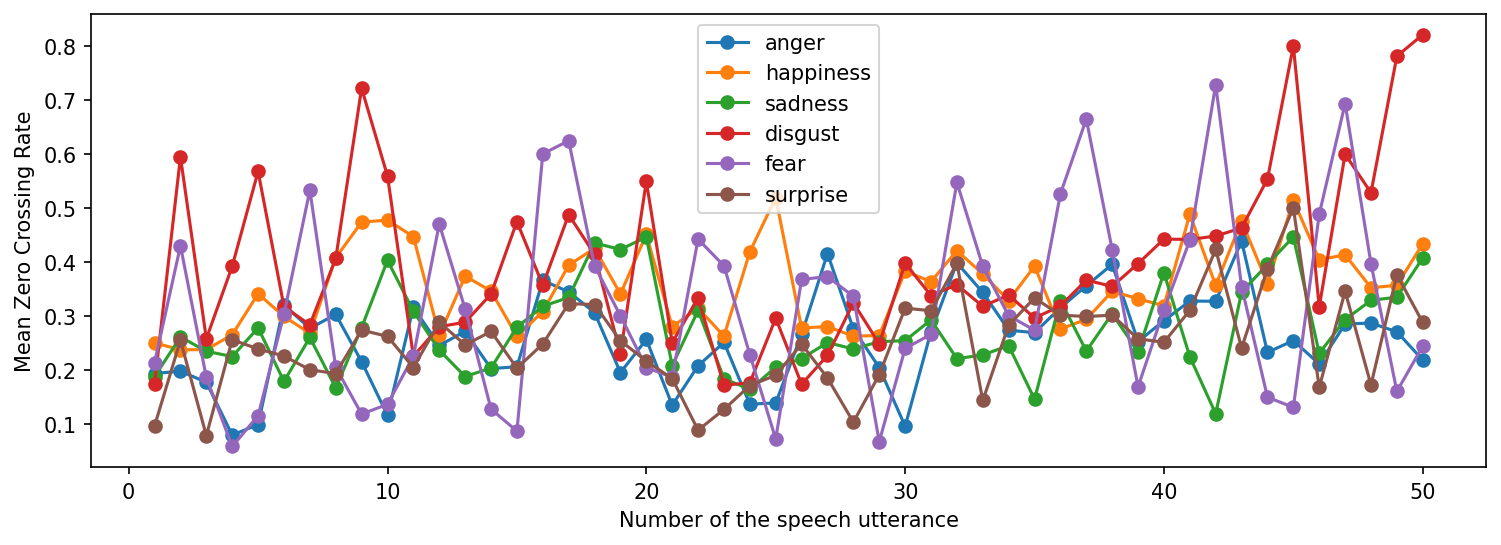
\includegraphics[width=\linewidth]{figs/4_1_traditional/meanZCRVar.png}
	\caption{Zero crossing rate mean values variation plot along 50 audios of speech utterances for all emotions}
	\label{fig:zcrMeanVar}
\end{figure}

A common observation for most extracted feature plots was that the values were not consistent across multiple audio segments for the same emotion. However, the number of audio segments used in this study was relatively low (only 50) to observe big variability changes, but increasing the number of audio segments would also make it more challenging to observe such variability through a simple visual inspection.

\subsubsection{Box Plots}

Finally, we employed box plots to visualize the distribution of the features on different subjects, as well as to compare the values for each emotion. An example of this type of plot is shown in Figure \ref{fig:zcrMeanBoxPlot}, which displays the mean zero crossing rate feature for all emotions and different subjects. 

\begin{figure}[H]
	\centering
	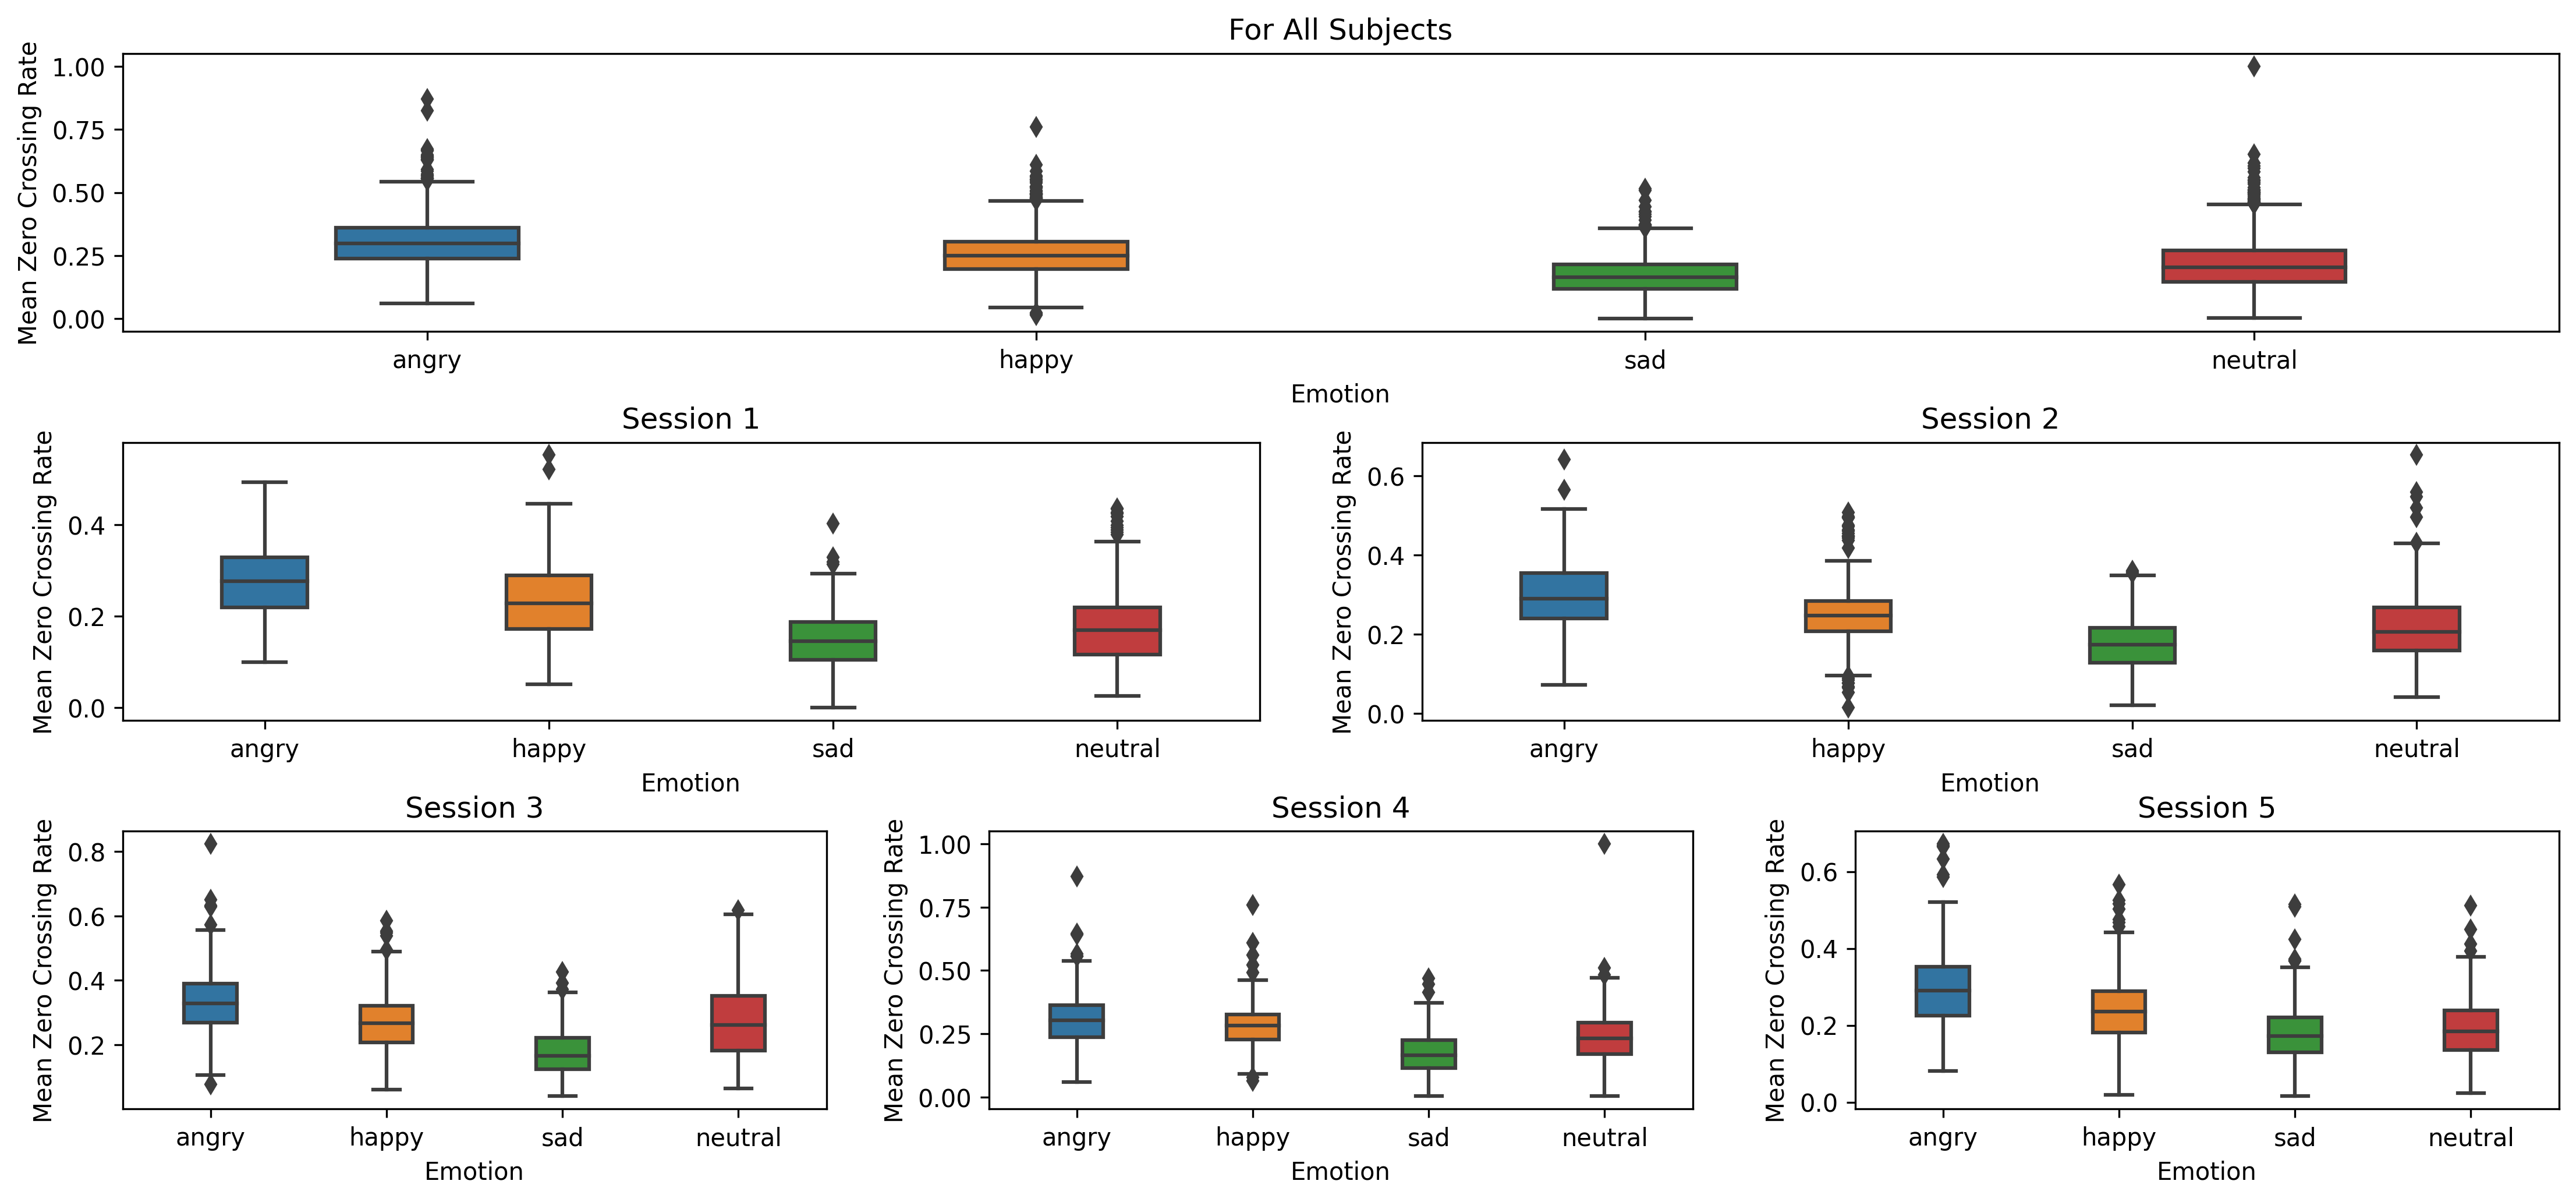
\includegraphics[width=\linewidth]{figs/4_1_traditional/mean_zcr_box_plot.png}
	\caption{Zero crossing rate mean values box plot for all emotions and different subjects}
	\label{fig:zcrMeanBoxPlot}
\end{figure}

The primary purpose of using these plots was to provide a simple and intuitive representation of each feature. By comparing the values across all subjects or a selected few, any noticeable differences in feature values for each emotion could be easily perceived.

\subsection{Feature Selection}

After the process of feature analysis, the next step in \ac{ser} development is feature selection. Feature selection is a technique to choose a subset of the original set of features that are most relevant for the given task. The process of feature selection is aimed to improve the accuracy of the model and reducing the problem's complexity by removing redundant or irrelevant features. 

The objective is to choose a smaller set of features that retain enough information for good classification performance while being computationally efficient. Hence, a smaller subset of features that can provide effective classification results is preferred over the larger set of features that may be computationally expensive and redundant.

\subsubsection{High Correlation Elimination}

Correlation among our extracted features is common since many of them use the same audio descriptor but with a different metric applied to them. Therefore, a correlation matrix for all 327 extracted features was calculated using the Pearson method, presented in the figure \ref{allAudioFeat}.

A high correlation elimination was performed by selecting every pair features with a Pearson correlation coefficient absolute value of 0.6 or above, then it was removed the feature with the highest average correlation value with all the other features. This process resulted in the elimination of 230 features, leaving 97 features for subsequent analysis. The correlation matrix after the feature selection process is presented in the figure \ref{fig:highAudioFeat}.

\begin{figure}
	\centering
	\begin{subfigure}{.5\textwidth}
		\centering
		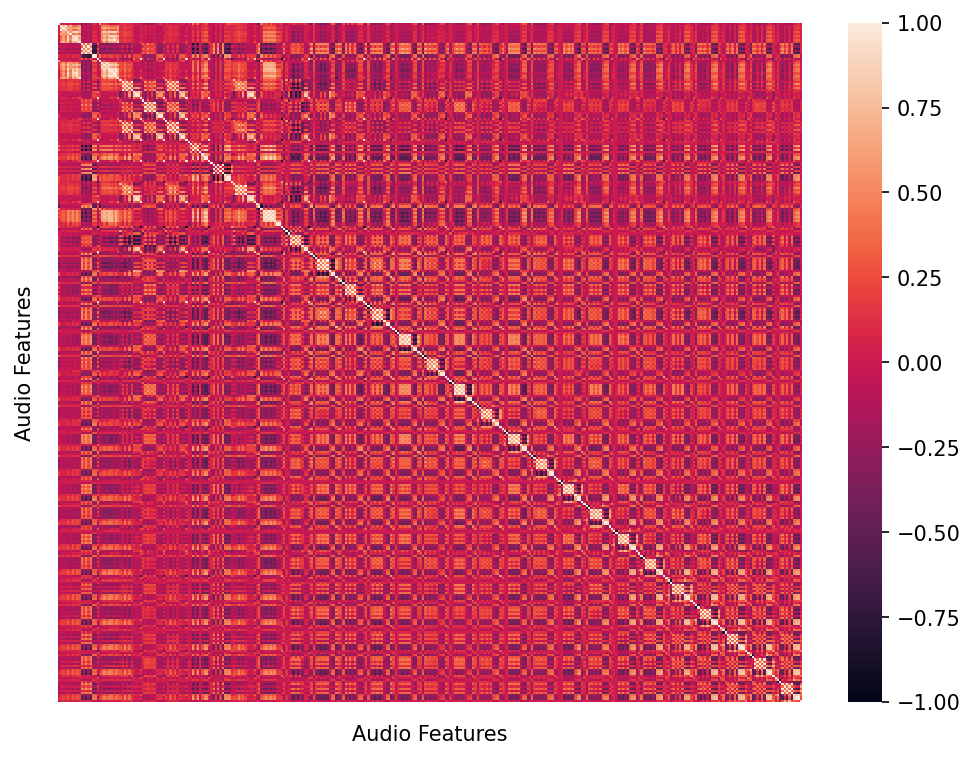
\includegraphics[width=\linewidth]{figs/4_1_traditional/allCorrMatrix.png}
		\caption{Correlation Matrix of all the Features.}
		\label{fig:allAudioFeat}
	\end{subfigure}%
	\begin{subfigure}{.5\textwidth}
		\centering
		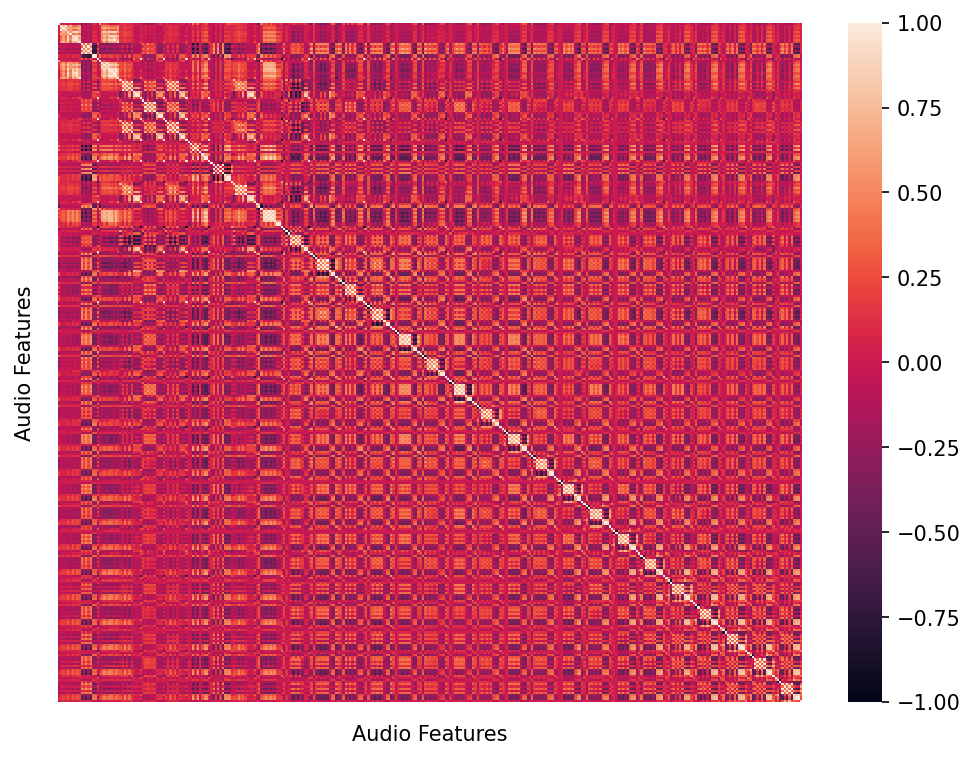
\includegraphics[width=\linewidth]{figs/4_1_traditional/highCorrMatrix.png}
		\caption{Correlation Matrix after High Correlation Elimination.}
		\label{fig:highAudioFeat}
	\end{subfigure}
	\caption{Audio Features' Pearson Correlation Matrices Before and After High Correlation Elimination.}
\end{figure}



\subsubsection{Selecting an Initial Classifier}

Along this process, it became necessary to choose a model to be used in computanioally expensive feature selection methods. Consequently, several estimators were tested for their performance in classifying emotions.

To this end, we conducted 5-fold cross-validation and compared the mean and standard deviation accuracies of all folds, as well as the total execution time for various classifiers from the scikit-learn library \cite{scikit-learn}, using the features obtained after the previous process, as shown in Table \ref{tab:modelsPerformance}.

\begin{table}[H]
	\caption{Performance of various classifiers in 5-fold cross-validation using the 97 features obtained after high correlation elimination.}
	\centering
	\label{tab:modelsPerformance}
	\begin{tabular}{lccc}
		\toprule
		Classifiers &   Mean Accuracies &   Standard Deviation Accuracies & Total Time (s)\\
		\midrule
		Ridge   &        0.652 &      0.024 & 0.038 \\
		Extra Trees   &        0.641 &      0.048 & 1.789 \\
		Random Forest &        0.629 &      0.028 & 4.529 \\
		XGBoost     &        0.619 &      0.037 & 2.456 \\
		AdaBoost   &        0.585 &      0.025 & 9.018 \\
		Decision Tree &        0.408 &      0.042 & 0.227 \\
		Extra Tree  &        0.364 &      0.045 & 0.026 \\
		C-Support Vector  &        0.329 &      0.046 & 0.202 \\
		Multi-layer Perceptron    &        0.301 &      0.035 & 0.716 \\
		\bottomrule
	\end{tabular}
\end{table}

Based on the evaluation results, the Ridge classifier was chosen for further analysis. This model exhibited the best prediction metrics and was also the fastest among all the evaluated classifiers. Therefore, it was deemed suitable for performing computationally expensive feature selection methods.


\subsubsection{Feature Elimination with Backwards Propagation}

In the pursuit of completing the feature selection process, a sequential feature selection with backward propagation was employed. This method involves performing a 5-fold cross-validation with the previously selected Ridge classifier, using all features except one, and then removes one feature based on the lowest mean accuracy of the 5 folds. This iterative process continues until only one feature remains.

A method was then developed to select the furthest highest accuracy. This method involves finding a maximum and multiplying it by a threshold value of $0.99$ to balance accuracy with the number of removed features. Figure \ref{fig:backProp1} displays the mean accuracies obtained at each step and the chosen furthest highest accuracy.

\begin{figure}[H]
	\centering
	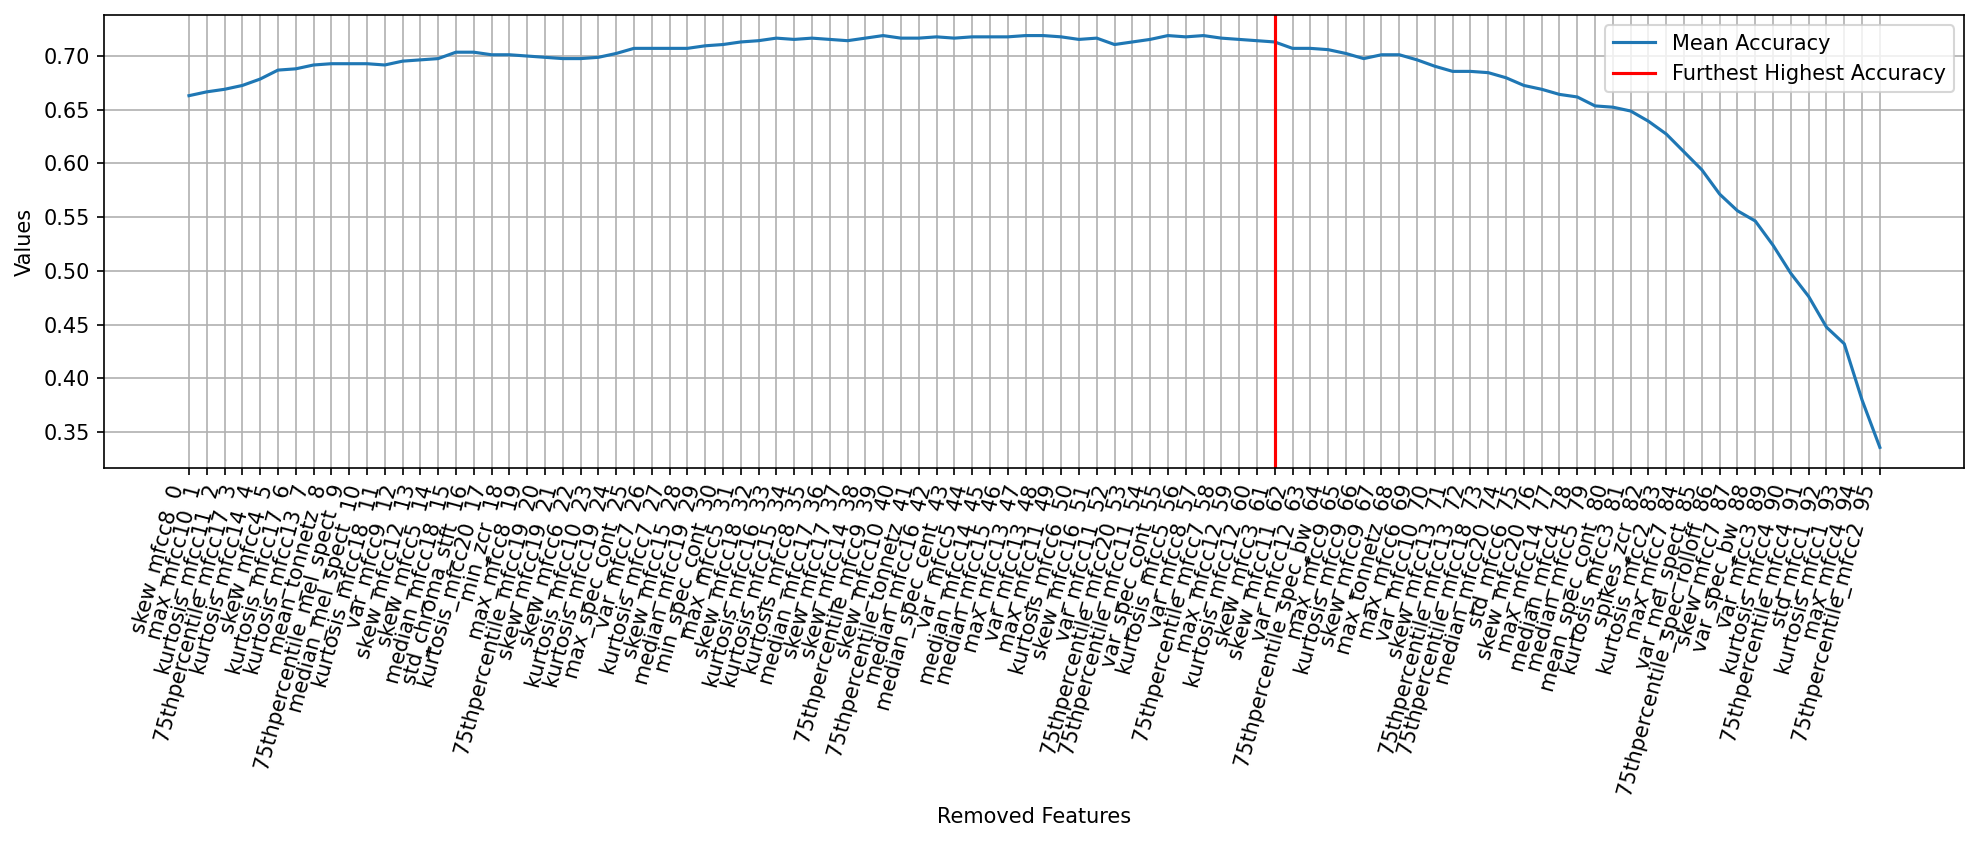
\includegraphics[width=1\linewidth]{figs/4_1_traditional/backProp1.png}
	\caption{Sequential Feature Selection with Backward Propagation using the Mean Accuracy as the Selection Method.}
	\label{fig:backProp1}
\end{figure}

This process led to the elimination of 62 features from the initial set of 97 obtained after the high correlation elimination, leaving a total of 35 features, as shown in Table \ref{tab:selectedFeat}.

\begin{table}[H]
	\caption{Selected features.}
	\centering
	\label{tab:selectedFeat}
	\resizebox{\textwidth}{!}{%
	\begin{tabular}{ll}
		\toprule
		Metric & Audio Features \\
		\midrule
		75th Percentile & MFCC-2, MFCC-4, MFCC-13, MFCC-18, Spectral Bandwidth, Spectral Roll-Off\\
		Variance & MFCC-3, MFCC-4, MFCC-10, MFCC-12, Spectral Bandwidth, Mel-Spectrogram\\
		Maximum & MFCC-4, MFCC-6, MFCC-7, MFCC-9, MFCC-14, Tonnetz\\
		Skew & MFCC-7, MFCC-9, MFCC-11, MFCC-13, MFCC-20\\
		Kurtosis & MFCC-1, MFCC-2, MFCC-3, MFCC-4, MFCC-9\\
		Median & MFCC-4, MFCC-5, MFCC-20\\
		Standard Deviation & MFCC-1, MFCC-6\\
		Mean & Spectral Contrast\\
		Spikes & Zero-Crossing-Rate\\
		\bottomrule
	\end{tabular}
	}
\end{table}



\subsubsection{Testing Classifiers}\label{metrics}

Finally, we intended to corroborate the quality of the feature selection. To do so, several evaluation metrics were calculated from the estimations: \begin{enumerate*}
	\item Accuracy
	\item Macro F1
	\item Precision
	\item Recall
	\item Hamming
	\item Matthews Correlation Coefficient (MCC)
\end{enumerate*}

A series of predictions were performed and plotted the confusion matrix of the predictions \ref{confusionMatrices}, furthermore, evaluation metrics were also calculated, as the table \ref{tab:acc} shows. 

In the first situation, a Random Forest model was trained with 194 of all the initial features (case 1), secondly, trained with the 50 features after the high correlation elimination (case 2), then, with the remaining 24 features after both the high correlation elimination, and, the feature elimination with backward propagation (case 3).

Moreover, one vs rest, also known as one vs all classifier, was implemented. This strategy consisted in fitting one Random Forest classifier per label. For each classifier, the label is fitted against all the other labels. For this strategy, it used all 194 initial features (case 4), and, the same of case 3, as input for each classifier (case 5).


\begin{table}[H]
	\caption{Predictions' Evaluations Metrics with Different Strategies and Input Data}
	\centering
	\label{tab:acc}
	\begin{tabular}{ccccccccc}
		\toprule
		Case & N.º of Features & Accuracy & Macro F1 & Precision & Recall & MCC. \\
		\midrule
		(1) & 194 & 0.461 & 0.453 & 0.456 & 0.461 & 0.354\\
		(2) &  50 & 0.417 & 0.408 & 0.411 & 0.417 & 0.302\\
		(3) &  24 & 0.417 & 0.411 & 0.413 & 0.417 & 0.302\\
		(4) & 194 & 0.450 & 0.440 & 0.443 & 0.450 & 0.342\\
		(5) &  24 & 0.433 & 0.424 & 0.426 & 0.433 & 0.321\\
		\bottomrule
	\end{tabular}
\end{table}


It is possible to observe from the table \ref{tab:acc}, that, there is some loss of accuracy from the first situation to the rest, and, the second and third situations have almost the same results. From this, if the short loss in prediction performance could be an acceptable price to pay. the third situation is optimal since there are 170 fewer features used as input data, therefore, speeding up the prediction calculation time.

In addition, the 4th case and 5th cases show similar results to the 1st case and 3rth cases respectively, so, it was concluded that using a one vs rest wasn't a good strategy, since the prediction performance wasn't improved a lot, and it increased the computational cost by using more classifiers.


\subsection{Conclusion}

During the feature analysis, most of the displayed graphs represent univariate studies of the features, therefore, if, visually, a feature is perceived as a bad descriptor, it doesn't invalidate its usage for the emotion classification problem, and it is essential to employ some other multivariate studies.

The data were also analyzed in terms of gender bias, by comparing the data of male and female subjects' audios, and, reasoned that the dataset does not contain sufficient data to take any well-founded conclusion.

\section{Classifiers Evaluation and Selection}